\documentclass{article}
\usepackage[margin=0.5in]{geometry}
\usepackage[utf8]{inputenc}

\usepackage[table]{xcolor}
\usepackage{graphicx}
\usepackage{array}
\def\Tab#1{\tabular[t]{>{\rule[-1ex]{0pt}{3ex}}c}#1\endtabular}
\newcolumntype{C}{@{}c@{}}

\usepackage{pgfplots}
\usepackage{makecell}
\usepackage{multirow}
\pgfplotsset{width=10cm,compat=1.9}
%\usepgfplotslibrary{external}
%\tikzexternalize
\begin{document}
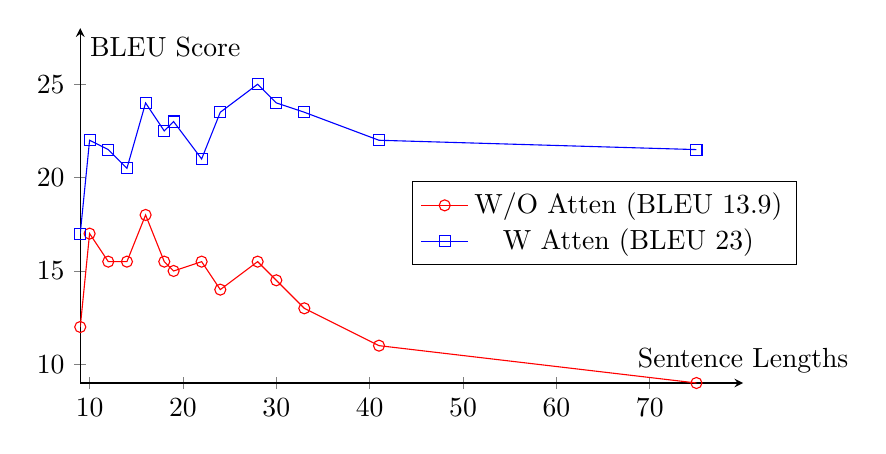
\begin{tikzpicture}
\begin{axis}[
    %title={Temperature dependence of CuSO$_4\cdot$5H$_2$O solubility},
    unit vector ratio*=1 2 1,
    axis lines=middle, enlargelimits=false,
    xlabel={Sentence Lengths},
    xlabel style={
        anchor=south,
        align=right
    },
    ylabel={BLEU Score},
    ylabel style={
        anchor=north west,
        align=right
    },
    xmin=9, xmax=80,
    ymin=9, ymax=28,
    xtick={10, 20, 30, 40, 50, 60 ,70},
    ytick={10, 15, 20, 25},
    legend style={at={(0.5,0.45)},anchor=west}
]
\addplot[
    color=red,
    mark=o,
    ]
    coordinates {
    (9, 12)(10, 17)(12, 15.5)(14, 15.5)(16, 18)(18, 15.5)(19, 15)(22, 15.5)(24, 14)(28, 15.5)(30, 14.5)(33, 13)(41, 11)(75, 9)
    };
    \addlegendentry{\text{W/O Atten (BLEU 13.9)}}
\addplot[
    color=blue,
    mark=square,
    ]
    coordinates {
    (9, 17)(10, 22)(12, 21.5)(14, 20.5)(16, 24)(18, 22.5)(19, 23)(22, 21)(24, 23.5)(28, 25)(30, 24)(33, 23.5)(41, 22)(75, 21.5)
    };
    \addlegendentry{\text{W Atten (BLEU 23)}}
 
\end{axis}
\end{tikzpicture}

\vspace{5cm}

\begin{table}[p]
\begin{tabular}{ @{}r@{} | C || C C C} 

\Tab{ \\ \Xhline{2\arrayrulewidth}
     \rotatebox{90}{~\parbox{0.58cm}{%
  En $\to$
}~} \\ \hline
 \rotatebox{90}{~\parbox{0.58cm}{%
  En $\gets$
}~}
}
&

\Tab{ \\ \Xhline{2\arrayrulewidth}
     Simultaneous GD \\[0.5ex] Baseline \\ \hline Simultaneous GD \\[0.5ex] Baseline}
&

\Tab{Cs \\ \Xhline{2\arrayrulewidth}
     15.2 \\[0.5ex] 13.84 \\ \hline 20.47 \\[0.5ex]  20.32}
&

\Tab{De \\ \Xhline{2\arrayrulewidth}
     19.5 \\[0.5ex] 21.75 \\ \hline 23.96 \\[0.5ex] 24}
&

\Tab{Ru \\ \Xhline{2\arrayrulewidth}
     17.77 \\[0.5ex] 19.54 \\ \hline 22.27 \\[0.5ex] 22.44}


\end{tabular}
\end{table}

\end{document}